\section{COCOMO Approach}
	Considering to use JEE as programming language, to pass from FP to SLOC we can use the average convertion factor 46, as described at the site \emph{http://www.qsm.com/resources/function-point-languages-table}. 
	$$SLOC=UFP*ConvertionFactor$$
	$$SLOC=72*46=3312$$
	
	According to the table below, we have considered the underlined values in yellow for the scale drivers and the underlined values in green for the cost drivers.
	
	\begin{center}
			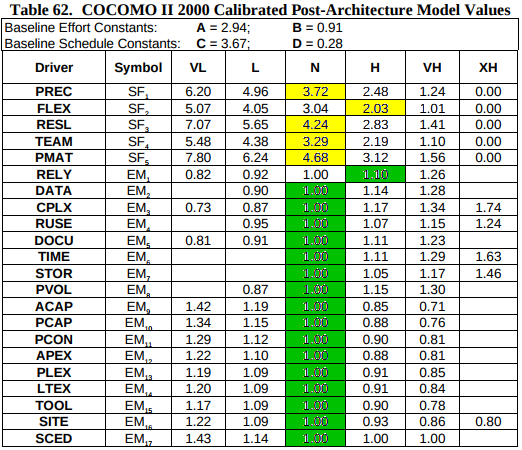
\includegraphics[width=0.95\textwidth]{./images/drivers.png}
	\end{center}
	
	Considering only the scale drivers, we make the following addition:
	$$E=B + 0.01*(PREC+FLEX+RESL+TEAM+PMAT)$$ where B = 0.91 for COCOMO-II
	$$E=0.91+0.01*(3.72+2.03+4.24+3.29+4.68)=1.0896$$
	
	
	Considering only the cost drivers, we make the following moltiplication:
	$$EAF=RELY*DATA*CPLX*RUSE*DOCU*TIME*STOR*PVOL*ACAP*PCAP*PCON*APEX*PLEX*LTEX*TOOL*SITE*SCED$$
	$$EAF=1.10*1.00*1.00*1.00*1.00*1.00*1.00*1.00*1.00*1.00*1.00*1.00*1.00*1.00*1.00*1.00*1.00=1.10$$
	
	So, now we can compute the effort, using the formula below:
	$$effort=2.94*EAF*(KSLOC)^E$$
	$effort=2.94*1.10*(3.312)^1.0896 = 11.92$ person/months
	
	\newline 
	Now we calculate the duration of the project in months, using the following formula:
	$$duration = C*(effort)^(D+0.2*(E-B))$$ where C = 3.67, D = 0.28, B = 0.91 for COCOMO-II
	$duration = 3.67*(11.92)^(0.31592) = 8.03$ months
	
	\newline
	The people needed to complete the project are calculated through the formula below:
	$$N_{people} = \ceil{effort/duration} $$
	$$N_{people} = \ceil{11.92/8.03} = \ceil{1.48} = 2$$
	
	Using the online tool {http://csse.usc.edu/tools/COCOMOII.php}, we give a more accurate estimation of the previous calculus. In the following images, we can see the results.  
	
	\begin{center}
			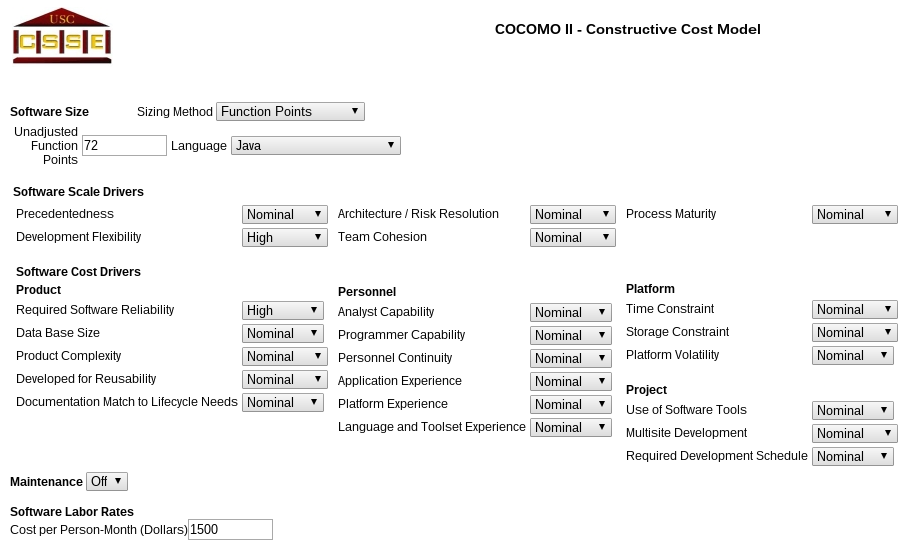
\includegraphics[width=0.95\textwidth]{./images/cocomo1.png}
	\end{center}
	
	\begin{center}
			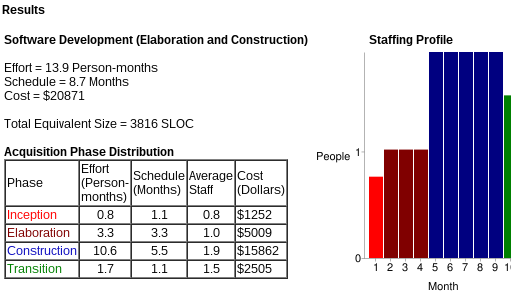
\includegraphics[width=0.95\textwidth]{./images/cocomo2.png}
	\end{center}
	 